Puntos a abordar

- mencionar realizabilidad clásica. Related work capaz en la conclusión
- hacer una investigación de otras formas de hacer witness extraction. Capaz no es original lo nuestro (y capaz Coq lo banca con realizabilidad).

\begin{itemize}
    \item Motivación, limitaciones de lógica clásica. Demostración sqrt 2
    \item Lógica intuicionista
    \item Como necesitamos reducir en ND, necesitamos la demo en ND. Escribirla
    en este caso.
    \item También queremos para $\classPiTwo$, mostrar la extensión en ND.
    \item En realidad no nos sirve $\transDNeg{\Gamma}$, queremos dejarlo como
    está y demostrar que los axiomas demuestran sus traducciones. Pero no vale
    siempre (buscar c.ej), caracterizar cuando.
    \item Sumarizar cómo queda, vincular con reducción. Mostrar ejemplos en PPA
    que funcionan y ejemplos que no.
    \item Extensión a demostraciones. Mostrar algunos ejemplos interesantes (y
    los que usen los lemas dNegRElim y rElim)
    \item Lemas para demostraciones: dNegRElim (relacionar con \ref{ppa-cert:sec:abs-reasoning}), rElim, tNegRElim
    \item Reducción (buena explicación
    \url{https://plato.stanford.edu/entries/natural-deduction/}). En realidad se
    conoce como \textbf{normalization}.
    \begin{itemize}
        \item Similitud con reducción en cálculo lambda.
        \item Ejemplos de LP y todo LPO
        \item substHyp, substVar en proofs
        \item Argumentos de que es correcto y completo?
        \item Small step vs big step
    \end{itemize}
\end{itemize}

\newpage

En los capítulos anteriores vimos como el lenguaje PPA puede ser usado para
escribir demostraciones de alto nivel, que son certificadas generando
demostraciones de bajo nivel usando el sistema lógico de deducción natural.
Ahora vamos a introducir una nueva funcionalidad: la \textbf{extracción de testigos}.

\begin{multicols}{2}
    \begin{figure}[H]
        \lstinputlisting{listings/extract/exists.ppa}
        \caption{Extracción simple}
        \label{fri:prog:exists}
    \end{figure}

    \begin{figure}[H]
        \lstinputlisting{listings/extract/forall.ppa}
        \caption{Extracción con instanciación}
        \label{fri:prog:forall}
    \end{figure}
    \begin{figure}[H]
        \lstinputlisting[firstline=2]{listings/extract/indirect.ppa}
        \caption{Extracción indirecta}
        \label{fri:prog:indirect}
    \end{figure}
\end{multicols}

Por ejemplo, en el programa \fullref{fri:prog:exists} la extracción nos
permitirá encontrar un término $t$ que sea testigo de $\exists x. p(x)$, es
decir que cumpla $p(t)$. En este caso es fácil encontrarlo a ojo sobre la
demostración de PPA, sería \lstinline{v}. Pero puede haber casos en donde no sea
tan trivial, como en el programa \fullref{fri:prog:indirect}, en donde se
instancia la variable en un término de forma indirecta. Además, también
querríamos poder extraer en casos donde haya cuantificadores universales, como
en \fullref{fri:prog:forall}. Buscamos un mecanismo general, que nos permita a
partir de cualquier demostración una fórmula de la pinta $\forall \var_0 \dots
\forall \var_n \exists \varTwo . \alpha$ extraer un testigo. Vamos a hacerlo a
partir de los certificados de deducción natural.

\section{La lógica clásica no es constructiva}

El objetivo es extraer el testigo de las demostraciones generadas por el
certificador, pero estas son en lógica clásica, que tiene el gran problema de
que en general, \textbf{no es constructiva}. ¿Qué quiere decir? Que en general,
puede suceder que una demostración de $\exists x . p(x)$ no nos diga quien es
$x$, y por lo tanto no podamos extraer un testigo. Esto es porque en la lógica
clásica vale el \textit{principio del tercero excluido} o LEM

\begin{prop}[LEM] Para toda fórmula $\form$, es verdadera ella o su negación
    \[ \form \fOr \fNot \form \]
\end{prop}

Las demostraciones que usan este principio suelen dejar aspectos sin
concretizar, como muestra el siguiente ejemplo bien conocido:

\begin{theorem}\label{fri:thm:irrat}
    Existen dos números irracionales, $a, b$ tales que $a^b$ es irracional
\end{theorem}
\begin{proof}
    Considerar el número $\sqrt{2}^{\sqrt{2}}$. Por LEM, es o bien racional o
    irracional.
    \begin{itemize}
        \item Supongamos que es racional. Como sabemos que $\sqrt{2}$ es
        irracional, podemos tomar $a=b=\sqrt{2}$.
        \item Supongamos que es irracional. Tomamos $a = \sqrt{2}^{\sqrt{2}}, b
        = \sqrt{2}$. Ambos son irracionales, y tenemos

        \[
            a^b
            = \left( \sqrt{2}^{\sqrt{2}} \right)^{\sqrt{2}}
            = \sqrt{2}^{\sqrt{2} \cdot \sqrt{2}}
            = \sqrt{2}^{2}
            = 2,
        \]

        que es racional.
    \end{itemize}
\end{proof}

La prueba no nos da forma de saber cuales son $a$ y $b$. Es por eso que en
general, en lógica clásica, tener una demostración de un teorema que afirma la
existencia de un objeto que cumpla cierta propiedad, no necesariamente nos da
una forma de encontrar tal objeto. Entonces tampoco vamos a poder extraer un
testigo.

En el caso de \fullref{fri:thm:irrat} elegimos demostrarlo de forma no
constructiva, pero existen formas constructivas de hacerlo \todo{citation
needed}. Pero hay casos en donde no.

\begin{ejemplo}[Demostración no constructiva]
    Si consideramos la fórmula
    \[
        \exists x . ((x = 1 \fAnd C) \fOr (x = 0 \fAnd \fNot C))
    \]
    y pensamos en $C$ como algo indecidible, por ejemplo \texttt{HALT},
    trivialmente podemos demostrarlo de forma no constructiva (LEM con $C \fOr
    \fNot C$) pero nunca de forma constructiva.
\end{ejemplo}

\section{Lógica intuicionista}

Como alternativa a la lógica clásica existe existe la lógica
\textbf{intuicionista}, que se puede definir como la lógica clásica sin LEM\footnote{Al no tener LEM, tampoco valen principios de razonamiento clásicos equivalentes,
como la eliminación de la doble negación.}. Al
no contar con ese principio, las demostraciones son constructivas. Esto permite
por un lado tener interpretaciones computacionales (como la \textit{BHK}) y
además que exista la noción de \textit{forma normal} de una demostración.
Existen métodos bien conocidos para reducir prueba hacia su forma normal con un
proceso análogo a una reducción de cálculo $\lambda$. 

Esto permite usar como estrategia de extracción la siguiente: normalizar la
demostración y obtener el testigo de la forma normal. En ella, se esperaría que
toda demostración de un $\exists$ sea mediante \ruleExistsI{}, explicitando el
testigo.

\section{Estrategia de extracción de testigos}

Queremos extraer testigos de las demostraciones generadas por el certificador de
PPA, pero son en lógica clásica. Sabemos que podemos hacerlo para lógica
intuicionista. ¿Cómo conciliamos ambos mundos? Existen métodos que permiten
\textit{embeber} la lógica clásica en la intuicionista. Uno de ellos es la
\textbf{traducción de Friedman} que se aborda en la siguiente sección. La
estrategia general entonces es la siguiente (esquematizada en \namedref{fri:fig:strat}), dada una demostración en PPA como
por ejemplo de \namedref{fri:prog:exists}:
\begin{enumerate}
    \item La certificamos generando una demostración clásica en deducción
    natural, usando el \modCertifier{}. Nos da un contexto con una demostración
    por teorema.
    \item Generamos una única demostración haciendo \textit{inline} de las demostraciones de otros teoremas citados, así cuando se reduce, se reduce la demostración completa y no una parte.
    \item Usamos la traducción de Friedman para obtener una demostración
    intuicionista de la misma fórmula.

    \textbf{Restricción}: La fórmula a demostrar debe ser de la forma
    $\forall \varTwo_0 \dots \forall \varTwo_n . \exists \var . \form$.
    \item Instanciamos las variables de los $\forall$ en términos proporcionados
    por el usuario, quedando una fórmula de la forma $\exists \var . \form$.
    \item Normalizamos la demostración.
    
    \textbf{Limitación}: No vamos a poder llevar cualquier demostración a su
    forma normal.

    \item Al ser una demostración normalizada de un $\exists$, debe comenzar con
    \ruleExistsI{}, que especifica el término que hace cierta la fórmula. Este
    es precisamente el testigo que estábamos buscando.

    \proofTreeExistsI
\end{enumerate}

En las siguientes secciones vemos en detalle la traducción de Friedman y la
normalización (o reducción) de demostraciones.

\begin{figure}
    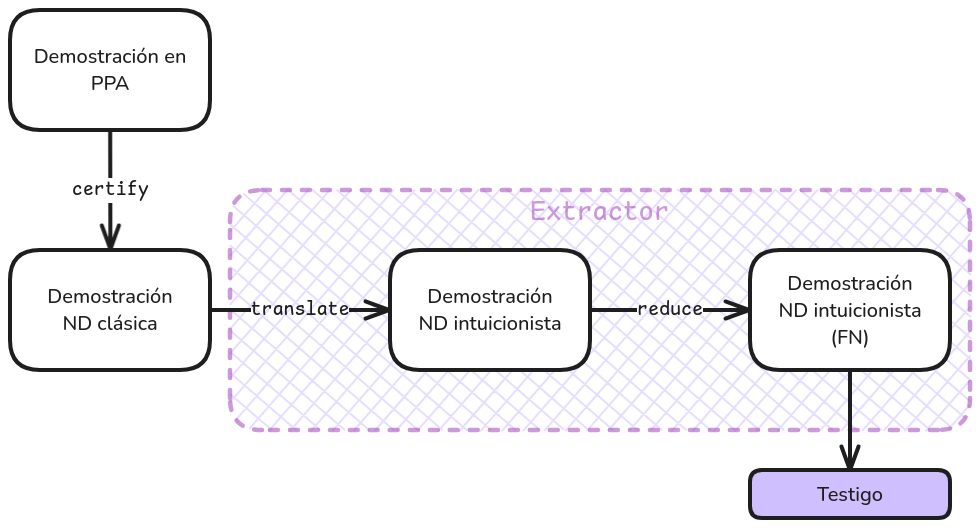
\includegraphics[scale=0.35]{img/fri-extract-strategy.png}
    \centering
    \caption{Estrategia de extracción de testigos}
    \label{fri:fig:strat}
\end{figure}

\section{Traducción de Friedman}

\subsection{Traducción de doble negación}

Existen muchos métodos que permiten embeber la lógica clásica en la
intuicionista \duda{citar?}. Un mecanismo general es la traducción de
\textbf{doble negación}, que tiene distintas variaciones. Una es la
\textit{Gödel-Gentzen} \cite{Avigad1998-FEFOFD}

\begin{definition}[Traducción \textit{Gödel-Gentzen}] Dada una fórmula $\form$
se asocia con otra $\gN{\form}$. La traducción se define por inducción
estructural.
    \begin{align*}
        \gN{\fFalse} &= \fFalse\\
        \gN{\fTrue} &= \fTrue\\
        \gN{\form} &= \fNot\fNot \form \quad \text{con $\form$ atómica}\\
        \gN{(\form \fAnd \formTwo)} &= \gN{\form} \fAnd \gN{\formTwo}\\
        \gN{(\form \fOr \formTwo)} &= \fNot(\fNot\gN{\form} \fAnd \fNot\gN{\formTwo})\\
        \gN{(\form \fImp \formTwo)} &= \gN{\form} \fImp \gN{\formTwo}\\
        \gN{(\forall \var . \form(\var))} &= \forall \var . \gN{\form(\var)}\\
        \gN{(\exists \var . \form(\var))} &= \fNot \forall \var . \fNot \gN{\form(\var)}
    \end{align*}
\end{definition}


\begin{definition}[Traducción de contextos]
    Se extiende a contextos de la forma esperable
    \[
        \gN{\ctx} = \{\gN{\form} \mid \form \in \ctx \}.
    \]
\end{definition}

\begin{notation*}
    Notamos,    
    \begin{itemize}
        \item $\judgC$ para expresar que un juicio es derivable en lógica clásica,
        y $\judgI$ para intuicionista.
        \item $\someProof \proves \ctx \judG \form$ para expresar que $\someProof$ es una demostración de $\ctx \judG \form$. Equivalente a
            \AxiomC{$\someProof$}
            \noLine
            \UnaryInfC{$\ctx \judG \form$}
            \DisplayProof
    \end{itemize}
\end{notation*}

\begin{theorem}
    Si tenemos $\ctx \judgC \form$, luego $\gN{\ctx} \judgI \gN{\form}$.
\end{theorem}

Dada una demostración en lógica clásica, podemos obtener una en lógica
intuicionista de su traducción. Pero esto no es exactamente lo que queremos,
pues si quisiéramos extraer un testigo de una demostración de la fórmula
$\exists \var. \pred(\var)$, al traducirla nos quedaría
\(
    \gN{(\exists \var. \pred(\var))}
        = \fNot \forall \var . \fNot\fNot\fNot \pred(\var),
\)
que si bien su demostración sería intuicionista (y por lo tanto constructiva),
como no es de un $\exists$ al normalizarla no podremos hacer la extracción.

\subsection{El truco de Friedman}

La idea de Friedman \cite{miquel-friedman} es generalizar la traducción
Gödel-Gentzen reemplazando la negación intuicionista $\fNot \form \equiv A
\rightarrow \bot$ por una relativa $\fNotR \form \equiv \form \rightarrow R$ que
está parametrizada por una fórmula arbitraria $R$. Esto nos va a permitir, con
una elección inteligente de $R$, traducir una demostración clásica de una
fórmula a una intuicionista, y usarla para demostrar \textbf{la fórmula
original}. Esto nos permite reducirla y hacer la extracción. No va a ser posible para cualquier fórmula, sino las de una clase particular (de la forma 
$\forall \varTwo_1 \dots \forall \varTwo_m . \exists \var_1 \dots \exists \var_k . \form$ o $\classPiTwo$)

\begin{definition}[Jerarquía aritmética de fórmulas]
    Clasifica las fórmulas en dos clases: $\classPi{n}$ y
    $\classSigma{n}$. Se define por inducción en $n$.

    \begin{itemize}
        \item Si $\anyForm$ es equivalente a una fórmula sin cuantificadores, está en
        $\classPi{0}$ y $\classSigma{0}$.
        \item Sean las clasificaciones $\classPi{n}$ y $\classSigma{n}$. Definimos para $n+1$.
        \begin{itemize}
            \item Si $\anyForm$ es equivalente a una formula de la forma $\exists
            \var_1 \dots \exists \var_k. \anyFormTwo$ donde $\anyFormTwo$ es
            $\classPi{n}$, entonces $\anyForm$ es asignada la clasificación $\classSigma{n+1}$.
    
            \item Si $\anyForm$ es equivalente a una formula de la forma $\forall
            \var_1 \dots \forall \var_k. \anyFormTwo$ donde $\anyFormTwo$ es
            $\classSigma{n}$, entonces $\anyForm$ es asignada la clasificación $\classPi{n+1}$.
        \end{itemize}
    \end{itemize}

    Una fórmula de $\classSigma{n}$ es equivalente a una que comienza con
    cuantificadores existenciales y alterna $n-1$ veces entre series de
    universales y existenciales. Mientras que una $\classPi{n}$ es análoga pero
    comenzando con universales.
    
    Las dos que más nos interesan son:
    \begin{itemize}
        \item $\classSigmaOne$: fórmulas de la pinta $\exists \var_1 \dots
        \exists \var_k . \anyForm$.
        \item $\classPiTwo$: fórmulas de la pinta $\forall \varTwo_1 \dots \forall \varTwo_m . \exists \var_1 \dots \exists \var_k . \anyForm$
    \end{itemize}

    

    Una intuición detrás de los nombres de las clases puede ser
    \begin{itemize}
        \item $\Sigma$ es una sumatoria, que se puede interpretar como
        disyunciones (en el sentido del álgebra de Boole), y generalizar con un existencial.
        \item $\Pi$ análogamente pero con productoria, conjunciones y universales.
    \end{itemize}
\end{definition}

\begin{definition}[Traducción de doble negación relativizada]
    \begin{align*}
        \transDNeg{\bot} &= \bot\\
        \transDNeg{\form} &= \fNotR\fNotR \form
            \quad \text{con $\form$ atómica}\\
        \transDNeg{(\fNot \form)} &= \fNot \transDNeg{\form}\\
        \transDNeg{(\form \fAnd \formTwo)} &= \transDNeg{\form} \fAnd \transDNeg{\formTwo}\\
        \transDNeg{(\form \fOr \formTwo)} &= \fNotR(\fNotR\transDNeg{\form} \fAnd \fNotR\transDNeg{\formTwo})\\
        \transDNeg{(\form \rightarrow \formTwo)} &= \transDNeg{\form} \rightarrow \transDNeg{\formTwo}\\
        \transDNeg{(\forall x . \form)} &= \forall x . \transDNeg{\form}\\
        \transDNeg{(\exists x . \form)} &= \fNotR \forall x . \fNotR \transDNeg{\form}
    \end{align*}
\end{definition}

\begin{theorem}
    \label{fri:thm:dneg-trans-classic-int}
    Si $\ctx \judgC \form$, luego $\transDNeg{\ctx} \judgI \transDNeg{\form}$
\end{theorem}
\begin{proof}
    Dada una demostración en deducción natural clásica $\ctx \judgC \form$, podemos traducirla recursivamente extendiendo la traducción de fórmulas a reglas de inferencia, así generando una demostración de $\transDNeg{\ctx} \judgI \transDNeg{\form}$.
    Este proceso está descrito en detalle en \fullref{fri:sec:proof-trans}
\end{proof}

Vamos a enunciar diferentes versiones de la traducción de Friedman en orden de sofisticación. No solo ayuda a entenderla, sino que también fue el mismo enfoque con el que las implementamos.

\begin{enumerate}
    \item \textbf{Fórmulas $\classSigmaOne$ atómicas} (\namedref{fri:thm:fri-sigmaone}):
    \[
        \exists \var . \form(\var) \text{ con } \form(\var) \text{ atómica.} 
    \]
    \item \textbf{Fórmulas $\classPiTwo$ atómicas} (\namedref{fri:thm:fri-pitwo}):
    
    \[
        \forall \varTwo_1 \dots \forall \varTwo_n . \exists \var . \form(\var, \varTwo_1, \dots, \varTwo_n) \text{ con } \form(\dots) \text{ atómica}.
    \]

    \item \textbf{Fórmulas $\classPiTwo$ no atómicas} (\namedref{fri:thm:fri-pitwo-general}):
    
    \[
    \forall \varTwo_1 \dots \forall \varTwo_n . \exists \var . \anyForm(\var, \varTwo_1, \dots, \varTwo_n) \text{ con } \anyForm(\dots) \text{ no atómica}.
    \]
    
    Por ejemplo, podría ser $\pred(x) \fAnd \predTwo(\varTwo_1, \dots, \varTwo_n)$.
    Pero no podrá ser cualquier fórmula, por ej. no $\fNot(\pred(x) \fAnd \predTwo(\varTwo_1, \dots, \varTwo_n))$. En \todo{Cita} damos una caracterización.
\end{enumerate}

\begin{theorem}[Traducción de Friedman para fórmulas $\classSigmaOne$]
    \label{fri:thm:fri-sigmaone}

    Sea $\someProof$ una demostración clásica de $\exists \var . \form$, y
    $\form$ una fórmula atómica.
    Si tenemos
    \[
        \ctx \judgC \exists \var . \form,
    \]
    luego, podemos generar una demostración intuicionista de \textit{la misma fórmula}
    \[
        \transDNeg{\ctx} \judgI \exists \var . \form.
    \]
\end{theorem}
\begin{proof}

Aplicando la traducción, tenemos que

\begin{gather*}
    \transDNeg{\big(
        \someProof \proves \ctx \judgC \exists \var . \form
    \big)}\\
    \verteq\\
    \transDNeg{\someProof} \proves \transDNeg{\ctx} \judgI \fNotR \forall \var . \fNotR \fNotR \fNotR \form
\end{gather*}

luego, tomando $R = \exists \var . \form$ la fórmula que buscamos probar,

\begin{align*}
    \transDNeg{\someProof} \proves & \transDNeg{\ctx} \judgI \fNotR \forall \var . \fNotR \fNotR \fNotR \form\\
    \iff & \transDNeg{\ctx} \judgI \fNotR \forall \var . \fNotR \form
        &&(\text{\namedref{fri:lemma:tnegr-elim}})\\
    =\ &\transDNeg{\ctx} \judgI (\forall \var . (\form \rightarrow R)) \rightarrow R
        &&(\fNotR \form = \form \fImp R)\\
    =\ &\transDNeg{\ctx} \judgI (\forall \var . (\form \rightarrow \exists \var . \form)) \rightarrow \exists \var . \form && (R = \exists \var \form)\\
    \Rightarrow\ &\transDNeg{\ctx} \judgI \exists \var . \form
        && (\text{\namedref{fri:obs:forall-exists}})
\end{align*}

En deducción natural,

\begin{prooftree}
    \def\defaultHypSeparation{\hskip .1in}
    \AxiomC{$\transDNeg{\someProof}$}
    \noLine
    \UnaryInfC{\(
        \transDNeg{\ctx} \judgI \fNotR \forall \var \fNotR \transDNeg{\form}
    \)}
    \AxiomC{}
    \RL{\ruleTNegRI}
    \admissibleRuleLine
    \UnaryInfC{$\transDNeg{\ctx}, \fNotR \form \judgI \fNotR \fNotR \fNotR \form$}
    \AxiomC{}
    \RL{\ruleAx}
    \UnaryInfC{$\transDNeg{\ctx}, \form \judgI \form$}
    \RL{\ruleExistsI}
    \UnaryInfC{$\transDNeg{\ctx}, \form \judgI R = \exists \var \form$}
    \RL{\ruleImpI}
    \UnaryInfC{$\transDNeg{\ctx} \judgI \fNotR \form$}
    \RL{\ruleCut}
    \admissibleRuleLine
    \BinaryInfC{$\transDNeg{\ctx} \judgI \fNotR \fNotR \fNotR \form$}
    \RL{\ruleForallI}
    \UnaryInfC{\(
        \transDNeg{\ctx} \judgI \forall \var \fNotR \transDNeg{\form}
    \)}
    \RL{\ruleImpE}
    \BinaryInfC{$\transDNeg{\ctx} \judgI \exists \var . \form$}
\end{prooftree}
\end{proof}

\begin{obs}
    En la demostración del \namedref{fri:thm:fri-sigmaone} y las de esta sección, luego de la traducción de Friedman, todas las demostraciones deben ser intuicionistas para que sigan siendo constructivas.
\end{obs}

\begin{lemma}[Eliminación de triple negación relativa]\label{fri:lemma:tnegr-elim}
    $\fNotR\fNotR\fNotR \form \iff \fNotR \form$ y lo demostramos como dos reglas admisibles, una para cada lado

    \begin{multicols}{2}
        \begin{prooftree}
            \AxiomC{}
            \RL{\ruleTNegRE}
            \admissibleRuleLine
            \UnaryInfC{$\fNotR\fNotR\fNotR \form \judgI \fNotR \form$}
        \end{prooftree}
    
        \begin{prooftree}
            \AxiomC{}
            \RL{\ruleTNegRI}
            \admissibleRuleLine
            \UnaryInfC{$\fNotR \form \judgI \fNotR\fNotR\fNotR \form$}
        \end{prooftree}
    \end{multicols}
\end{lemma}
\begin{proof}

    Primero \ruleTNegRI{}

    \begin{prooftree}
        \AxiomC{}
        \RL{\ruleAx}
        \UnaryInfC{$\fNotR \form, \fNotR\fNotR \form \judgI \fNotR \fNotR \form$}
        \AxiomC{}
        \RL{\ruleAx}
        \UnaryInfC{$\fNotR \form, \fNotR\fNotR \form \judgI \fNotR \form$}
        \RL{\ruleImpE}
        \BinaryInfC{$\fNotR \form, \fNotR\fNotR \form \judgI R$}
        \RL{\ruleImpI}
        \UnaryInfC{$\fNotR \form \judgI \fNotR\fNotR\fNotR \form$}
    \end{prooftree}

    Ahora \ruleTNegRE{}

    \begin{prooftree}
        \AxiomC{}
        \RL{\ruleAx}
        \UnaryInfC{$\fNotR\fNotR\fNotR \form, \form \judgI \fNotR\fNotR\fNotR \form$}
        \AxiomC{}
        \RL{\ruleAx}
        \UnaryInfC{$\ctx \judgI \fNotR \form$}
        \AxiomC{}
        \RL{\ruleAx}
        \UnaryInfC{$\ctx \judgI \form$}
        \RL{\ruleImpE}
        \BinaryInfC{$\ctx = \fNotR\fNotR\fNotR \form, \form, \fNotR \form \judgI R$}
        \RL{\ruleImpI}
        \UnaryInfC{$\fNotR\fNotR\fNotR \form, \form \judgI \fNotR\fNotR \form$}
        \RL{\ruleImpE}
        \BinaryInfC{$\fNotR\fNotR\fNotR \form, \form \judgI R$}
        \RL{\ruleImpI}
        \UnaryInfC{$\fNotR\fNotR\fNotR \form \judgI \fNotR \form$}
    \end{prooftree}
\end{proof}

\begin{obs}\label{fri:obs:forall-exists}
    $\judgI \forall \var (\form \rightarrow \exists \var \form)$.
    Trivialmente, para cualquier $\var$ si vale $\form$ entonces va a existir un $\var$ tal que valga $\form$.
\end{obs}

\todo{IDem pero en ND, y también para $\forall$}


\begin{theorem}[Traducción de Friedman para fórmulas $\classPiTwo$ atómicas]
    \label{fri:thm:fri-pitwo}

    Sea $\someProof$ una demostración clásica de
    \(
        \forall \varTwo_1 \dots \forall \varTwo_n .
        \exists \var .
        \form(\var, \varTwo_1, \dots, \varTwo_n)
    \)
    y $\form(\dots)$ una fórmula atómica

    Si tenemos
    \[
        \ctx \judgC
        \forall \varTwo_1 \dots \forall \varTwo_n .
        \exists \var .
        \form(\var, \varTwo_1, \dots, \varTwo_n),
    \]
    podemos generar una demostración intuicionista de la misma fórmula
    \[
        \transDNeg{\ctx} \judgI
        \forall \varTwo_1 \dots \forall \varTwo_n .
        \exists \var .
        \form(\var, \varTwo_1, \dots, \varTwo_n).
    \]
\end{theorem}
\begin{proof}
    \todo{proof}
\end{proof}

\subsubsection{Formulas no atómicas}
Es igual al anterior, pero para una fórmula arbitraria. Queremos generalizar r intro. Lema

\begin{lemma}[Introducción de $\fNotR$]
    No vale siempre.
\end{lemma}

\begin{theorem}[Traducción de Friedman para fórmulas $\classSigmaOne$ en general]
    \label{fri:thm:fri-pitwo-general}

    Sea $\someProof$ una demostración clásica de\(
        \forall \varTwo_1 \dots \forall \varTwo_n .
        \exists \var .
        \anyForm(\var, \varTwo_1, \dots, \varTwo_n)
    \), y
    $\anyForm(\var, \varTwo_1, \dots, \varTwo_n)$ una fórmula no atómica.
    Si tenemos
    \[
        \ctx \judgC 
        \forall \varTwo_1 \dots \forall \varTwo_n .
        \exists \var .
        \anyForm(\var, \varTwo_1, \dots, \varTwo_n),
    \]
    podemos generar una demostración intuicionista de la misma fórmula
    \[
        \transDNeg{\ctx} \judgI
        \forall \varTwo_1 \dots \forall \varTwo_n .
        \exists \var .
        \anyForm(\var, \varTwo_1, \dots, \varTwo_n).
    \]
\end{theorem}
\begin{proof}
    \todo{}
\end{proof}

\subsection{Traducción de demostraciones}
\label{fri:sec:proof-trans}

En \fullref{fri:thm:dneg-trans-classic-int} se introduce la necesidad de extender la traducción de doble negación relativizada de fórmulas a demostraciones, para poder convertir una demostración clásica a intuicionista. En esta sección lo vemos más en detalle.

La conversión se efectúa por inducción estructural en la demostración. Para cada regla de inferencia que demuestra $\form$, se genera una demostración a partir de ella para demostrar $\transDNeg{\form}$. La estrategia para hacerlo es similar para todas: usar la hipótesis inductiva para convertir las sub-demostraciones, y usarlas para generar la nueva demostración. Pero hay algunas que requieren un truco. Solo mostramos las interesantes.

\begin{itemize}
    \item \ruleAndI{} (\namedref{fri:lemma:trad-and-i}), \ruleAndEOne{}, \ruleAndETwo{}, \ruleImpI{}, \ruleImpE{}, 
    \ruleOrIOne{}, \ruleOrITwo{}, \ruleForallI{}, \ruleForallE{}, \ruleNotI{}, \ruleNotE{}, \ruleTrueI{}, \ruleAx{} son todas similares entre sí, por lo que solo mostramos una.
    \item \ruleExistsI{} (\namedref{fri:lemma:trad-exists-i}) es una regla simple pero más interesante que las anteriores, por la traducción de $\exists$.
    \item \ruleLEM{} (\namedref{fri:lemma:trad-lem}) es sumamente interesante, ya que se encuentra en el corazón de la traducción al ser la parte clave: ¿cómo traducimos el principio de razonamiento clásico que lo separa de la lógica intuicionista?
    \item \ruleFalseE{} (\namedref{fri:lemma:trad-false-e})  se prueba como lema por inducción estructural en la fórmula a demostrar.
    \item \ruleOrE{} (\namedref{fri:lemma:trad-or-e}) y \ruleExistsE{} son análogos y requieren un truco: usar la eliminación de la doble negación. Si bien al ser un principio de razonamiento clásico no vale para lógica intuicionista (por ser equivalente a LEM), lo que si vale es la eliminación de la doble negación relativizada: \ruleDnegRE{} (\namedref{fri:lemma:dnegr-e}).
\end{itemize}

\begin{lemma}[Traducción de \ruleAndI{}]
    \label{fri:lemma:trad-and-i}
    Dada una aparición de la regla \ruleAndI{},

    \begin{prooftree}
        \AxiomC{$\someProof_\form$}
        \noLine
        \UnaryInfC{$\ctx \judgI \form$}
        \AxiomC{$\someProof_\formTwo$}
        \noLine
        \UnaryInfC{$\ctx \judgI \formTwo$}
        \RL{\ruleAndI}
        \BinaryInfC{$\ctx \judgI \form \wedge \formTwo$}
    \end{prooftree}

    es posible traducirla generando una demostración de $\tdn{(\form \fAnd \formTwo)} = \tdn{\form} \fAnd \tdn{\formTwo}$.
\end{lemma}
\begin{proof}
    Por hipótesis inductiva, tenemos que
    \begin{itemize}
        \item \(
            \tdn{\someProof_\form} \proves
            \tdn{\ctx} \judgI
            \tdn{\form}
        \) y
        \item \(
            \tdn{\someProof_\formTwo} \proves
            \tdn{\ctx} \judgI
            \tdn{\formTwo}
        \)
    \end{itemize}

    Luego, podemos generar una demostración de $\tdn{\form} \fAnd \tdn{\formTwo}$

    \begin{prooftree}
        \AxiomC{$\tdn{\someProof_\form}$}
        \noLine
        \UnaryInfC{$\tdn{\ctx} \judgI \tdn{\form}$}
        \AxiomC{$\tdn{\someProof_\formTwo}$}
        \noLine
        \UnaryInfC{$\tdn{\ctx} \judgI \tdn{\formTwo}$}
        \RL{\ruleAndI}
        \BinaryInfC{$\tdn{\ctx} \judgI \tdn{\form} \fAnd \tdn{\formTwo}$}
    \end{prooftree}
\end{proof}

\begin{lemma}[Traducción de \ruleExistsI{}]
    \label{fri:lemma:trad-exists-i}
    \todo{Enunciar y demostrar}
\end{lemma}

\begin{lemma}[Traducción de \ruleLEM{}]
    \label{fri:lemma:trad-lem}
    \todo{Enunciar y demostrar}
\end{lemma}

\begin{lemma}[Traducción de \ruleFalseE{}]
    \label{fri:lemma:trad-false-e}
    \todo{Enunciar y demostrar}
\end{lemma}

\begin{lemma}[Eliminación de doble negación relativizada (\ruleDnegRE{})]
    \label{fri:lemma:dnegr-e}
    \todo{Enunciar y demostrar}
\end{lemma}

\begin{lemma}[Traducción de \ruleOrE{}]
    \label{fri:lemma:trad-or-e}
    \todo{Enunciar y demostrar}
\end{lemma}

\subsection{Manteniendo el contexto}

Problema con normalización: axiomas, hay que traducirlos para que la traducción de Friedman funcione. Solución? Dejar los axiomas originales y demostrar su traducción. No funciona siempre.

\begin{lemma}[Introducción de la traducción $\fNot\fNot$]
    Se reduce a transintro
\end{lemma}

\todo{Enunciar y demostrar}

\section{Normalización}

existe curry howard \cite{curry-howard-isomorphism}, relación entre deducción
natural y cálculo lambda. Luego, la normalización de demostraciones es el
isomorfismo de la semántica del cálculo lambda.

evitar \textit{detours}, leer más en el libro de curry howard

Mostrar ejemplo del and de curry howard.

\subsection{Sustituciones}

substHyp y substVar, la especificación matemática (y descripción de los problemas)

\subsection{Reglas de reducción}

Mostrar un par que sean intersantes, no todas.

\subsection{Estrategia de reducción}

...

\subsection{Limitaciones}

No funciona para todas las demostraciones, porque hay algunas reducciones que no implementamos.

\section{Otros métodos de extracción}

\todo{Hablar sobre y citar classical realizability, no tengo ni idea.}

Buena intro acá https://www.degruyter.com/document/doi/10.1515/9783110324921.11/html?lang=en

In the past years, many computational interpretations of Classical Arithmetic havebeen put forward.  Under a first classification, they fall into two large categories:directandindirectinterpretations.   Among  the  indirect  interpretations  one  findsthe  negative  translations  followed  either  by  Dialectica  interpretations  [13],  [30](see e.g.   Kohlenbach [19]) or by intuitionistic realizability interpretations com-bined with Friedman’s translation [13] (see e.g. Berger and Schwichtenberg [10]).Among the direct interpretations, there are different versions of Classical Realiz-ability (Krivine’s [22] and Avigad’s [6]), there is Coquand game semantics [11],